\chapter{Discussions}\label{chp7:discussions}
\begin{remark}{Outline}
If the populations of solitary ground nesting bees can be estimated by the number of active nests in a community, then the number of active nests can be manually counted. Over time manual counts can provide a measure of the changes in populations within a community. This method is comparatively straightforward and easy to replicate. Given this, it is reasonable to expect the number of active nests can also be counted from digital images of actual nests in much the same manner as manual estimations. If the number of active nests in an image can be counted, it is therefore also feasible to use image analysis to automatically identify the objects in the images that represent active nests. This reasoning was tested by using a practical monitoring program which was designed to collect manual nest counts and images of active nests for comparative analysis and proof of concept. Monitoring was conducted of over five years, at three communities of native bees in Whangarei (New Zealand). A total of 1896 images were collected representing 158 monitoring days. They were processed and used in a comparative analysis against manual field nest counts. This Chapter discusses the design, implementation and final performance evaluation of the image-centric nest monitoring system.
\end{remark}

\section{Research overview}
This study was based on the assumptions that, (1) the number of active nests could provide a proxy for populations and, (2) it was possible to design methods to reliably count the number of active nests at communities of bees over space and time, (3) that digital images could be used in the place of manual visual counts, (4) it was possible to process digital images to reliably count active nests. \marginpar{Background context, rationale, design methodology and research outcomes.} The evidence supporting the central ecological hypothesis that \emph{active nests of solitary ground nesting bees can provide a good proxy measure for populations} was taken from just a few studies \cite{Bischoff2003,Cane2008,Fellendorf2004}. There was no attempt to test this in the field. If time and resources had permitted, emergence traps and mark release recapture methods could have been implemented alongside manual nest counts and digital image acquisition. This could have provided sufficient data to test the \emph{active nest population proxy} hypothesis, but may have also been beyond the scope of this technology-based research. Furthermore, the field methods used in this research were designed towards a comparative analysis between manual and image-centric nest counts. Exactly the same nests were monitored over time. This approach would not met the criteria required for ecological field research because nest counts were not taken from randomly selected locations within or between native bee communities.

Since this research was primarily technology based, an image-based active nest counting pipeline could have been developed using pre-existing digital image samples collected during previous studies \cite{Hart2004,Hart2007}. The imaging design did not depend on actual long term field monitoring, manual nest counts or new image collections. From a broader perspective, there was little value in designing the image-centric monitoring system if it was not going to be recognised as a potential tool to aid ecological research. From a review of current literature there are many promising tools that have been developed for ecological research but for one reason or another, are underutilised in practical applications \cite{Potamitis2006,Raman2007,Batista2011}. In light of this and  contrary to the suggestions by Lindenmayer and Likens \cite{Lindenmayer2013} there was good motivation to test the image-centric monitoring system by gathering and using real field data. Furthermore, the design of this research was not context-free or based on retrofitted questions \cite{Lindenmayer2013}. It was founded on natural history observations of communities of native bees in Whangarei, recorded every year for over ten years \cite{Hart2004,Hart2007}. Thousands of hours of empirical observations have contributed towards a substantial understanding of native bees and their communities. This knowledge has included the challenges involved with monitoring them and the types of technologies that were best suited to aid in a greater scientific understanding of their communities and populations. Although the field methods used in this thesis are based on untested assumptions about the nest-proxy hypothesis, and they could have been improved to support a more rigorous scientific outcome by randomising sample collections, the image meta-data analysis used in this thesis could not be described as parasitic \cite{Lindenmayer2013}. However, it is also necessary to point out that if the number of active nests do not provide a good proxy for populations then the image-centric monitoring system outlined in this research is valuable for measuring the changes in active nests only. This was an issue that should have been properly tested when the research methodology was being designed. It is an issue that could have significant implications on the overall outcomes of this study because the wider scientific benefits of the nest monitoring system could be limited. The remaining discussions in this Chapter are therefore primarily concerned with design aspects of the image-centric monitoring system, as it was applied to measure the number of active nests rather than questioning the premise of nest-proxy measurements.

Open source tools were selected for nest image analysis to encourage community engagement in ecological research \cite{Hampton2013}. The processing pipeline and imaging methods are described in detail so they can be replicated. The core image analysis technique was based on trainable segmentations. Traditional segmentation techniques are \emph{repeatable} and reliable but are they only appropriate if the intensity values delineating target objects are well defined. Monitoring images were highly variable and the pixel areas representing active nests were not easily defined. Therefore classical segmentation techniques were not appropriate. In the past there were few alternatives to classical methods, but there are new techniques based on interactive machine learning. Therefore nest image segmentations were achieved using a semi-supervised machine learner and the \ac{TWS} workbench. Compared to classical binarization methods it would be difficult to exactly replicate the machine learning image segmentations used in this thesis. Therefore the procedures developed and used to optimise, train and apply machine learning classifiers for segmentations of active nest images in \ac{TWS} are described in detail. The image processing scripts, raw field and image data are also provided via Github for re-analysis or for use future research.

When the performance of the image-centric monitoring system was benchmarked against manual field counts the results were promising. Analysis showed the number of nests counted from images visually or by image analysis procedures, compared favourably with those from manual counts. The final monitoring results presented provided a reliable estimation of the number of active nests at the communities evaluated and the changes in nest numbers over time. However, as previously stated, because collection data was not randomly sampled the monitoring results from this study cannot be used as a proxy for native bee populations at the selected communities. Nevertheless, this research provided good evidence to show the populations of native bees could be reliably measured by using the image-centric monitoring method outlined in this thesis. In the future nest image data could be collected using proper random sampling methods thus providing data that could be used for a more rigorous scientific analysis. Field sampling methods would have little impact on the performance of the image-centric monitoring system. If the number of active nests can be manually counted in the field, then they can be estimated from images using the image-centric monitoring system with good agreement, accuracy and precision. The imaging method would stand alone and would not depend on collecting manual nest count data. It would also be possible to modify aspects of the image acquisition methods to incorporate remote imaging technology. This would reduce the dependence on manual labour and increase data capture for the scientific community.

\section{Active nests}
There were other \emph{types} of images that could have been used to reflect either the population changes over time or the species diversity of native bees within selected communities. \marginpar{Design of field methods, images of active nests and the alternative approaches?}This thesis has focused on the monitoring images of active nests. However, there were a range of image types were collected during field monitoring to test image acquisition techniques and image analysis procedures. This included capturing images of insects foraging on single flower heads (e.g. Figure \ref{fig:seq-image} (a)--(b)), insect clusters in flight around shrubs (e.g. Figure \ref{fig:measures-image} (b)), insect sweep net collections (e.g. Figure \ref{fig:measures-image}), active nests captured with and without grid quadrant (e.g. Figure \ref{fig:wideclose-image} and Figure \ref{fig:signs-image}). Active nests were the basis for the image-centric method presented in this thesis for the following reasons:

\begin{enumerate}
\item The images of active nests were easy to \emph{capture}.
\item The image area was easy to \emph{regulate}.
\item The image analysis required only \emph{two objects} to be segmented.
\item The results from analysis provided nest counts.
\item Nest counts could be directly used to measure populations.
\end{enumerate}

Nest images were relativity easy to capture when compared to moving insects (e.g. Figure \ref{fig:seq-image} (b)). Image acquisition was easier to govern for active nest data. This was achieved by using a standard of measure placed over an area of active nests. This was used to determine the focal boundaries of digital images.
The image analysis methods required to segment active nest images were not as complicated
as they were for other images. Some of the images would have required several target features to be segmented. For example, in Figure \ref{fig:seq-image} (b) six different insects are shown on single flower heads. The images were captured within a set time-frame and equate to a survey method that could be used for biodiversity sampling. The imaging pipeline for these types of images would have involved identifying at least six types of insects. Therefore the segmentation task would have been to partition the images into six key objects. In contrast to this there were only two categories in the  images of active nests that were necessary to segment; active nests from other backgrounds. Furthermore, image analysis based on the number of active nests in the images directly relates to an estimate of the populations of bees with minimal post-processing or statistical analysis. Thus compared to other image-types the images of active nests were much easier to capture, process and analyse. 

\begin{figure}[!htbp]\myfloatalign
\subfloat[Visitors to the same plant within a five minute time-frame.]{\includegraphics[width=1\linewidth]{gfx7/forage/f1}} \\
\subfloat[All the visitors to plants in a meter square.]{\includegraphics[width=1\linewidth]{gfx7/forage/f3}} \\
\caption[Image sequences of foraging bees.]{Image sequences of foraging bees and other insects focusing (a) on the same plant in a set time-frame and (b) on all plants and insects in a set area.}\label{fig:seq-image}
\end{figure}

\begin{figure}[!htbp] \myfloatalign
\subfloat[Image of a sweep net collection.]{\includegraphics[width=1\linewidth]{gfx7/collections/c2}} \\
/\subfloat[Grids for active nests (left) and a sphere for bees in flight (right).]{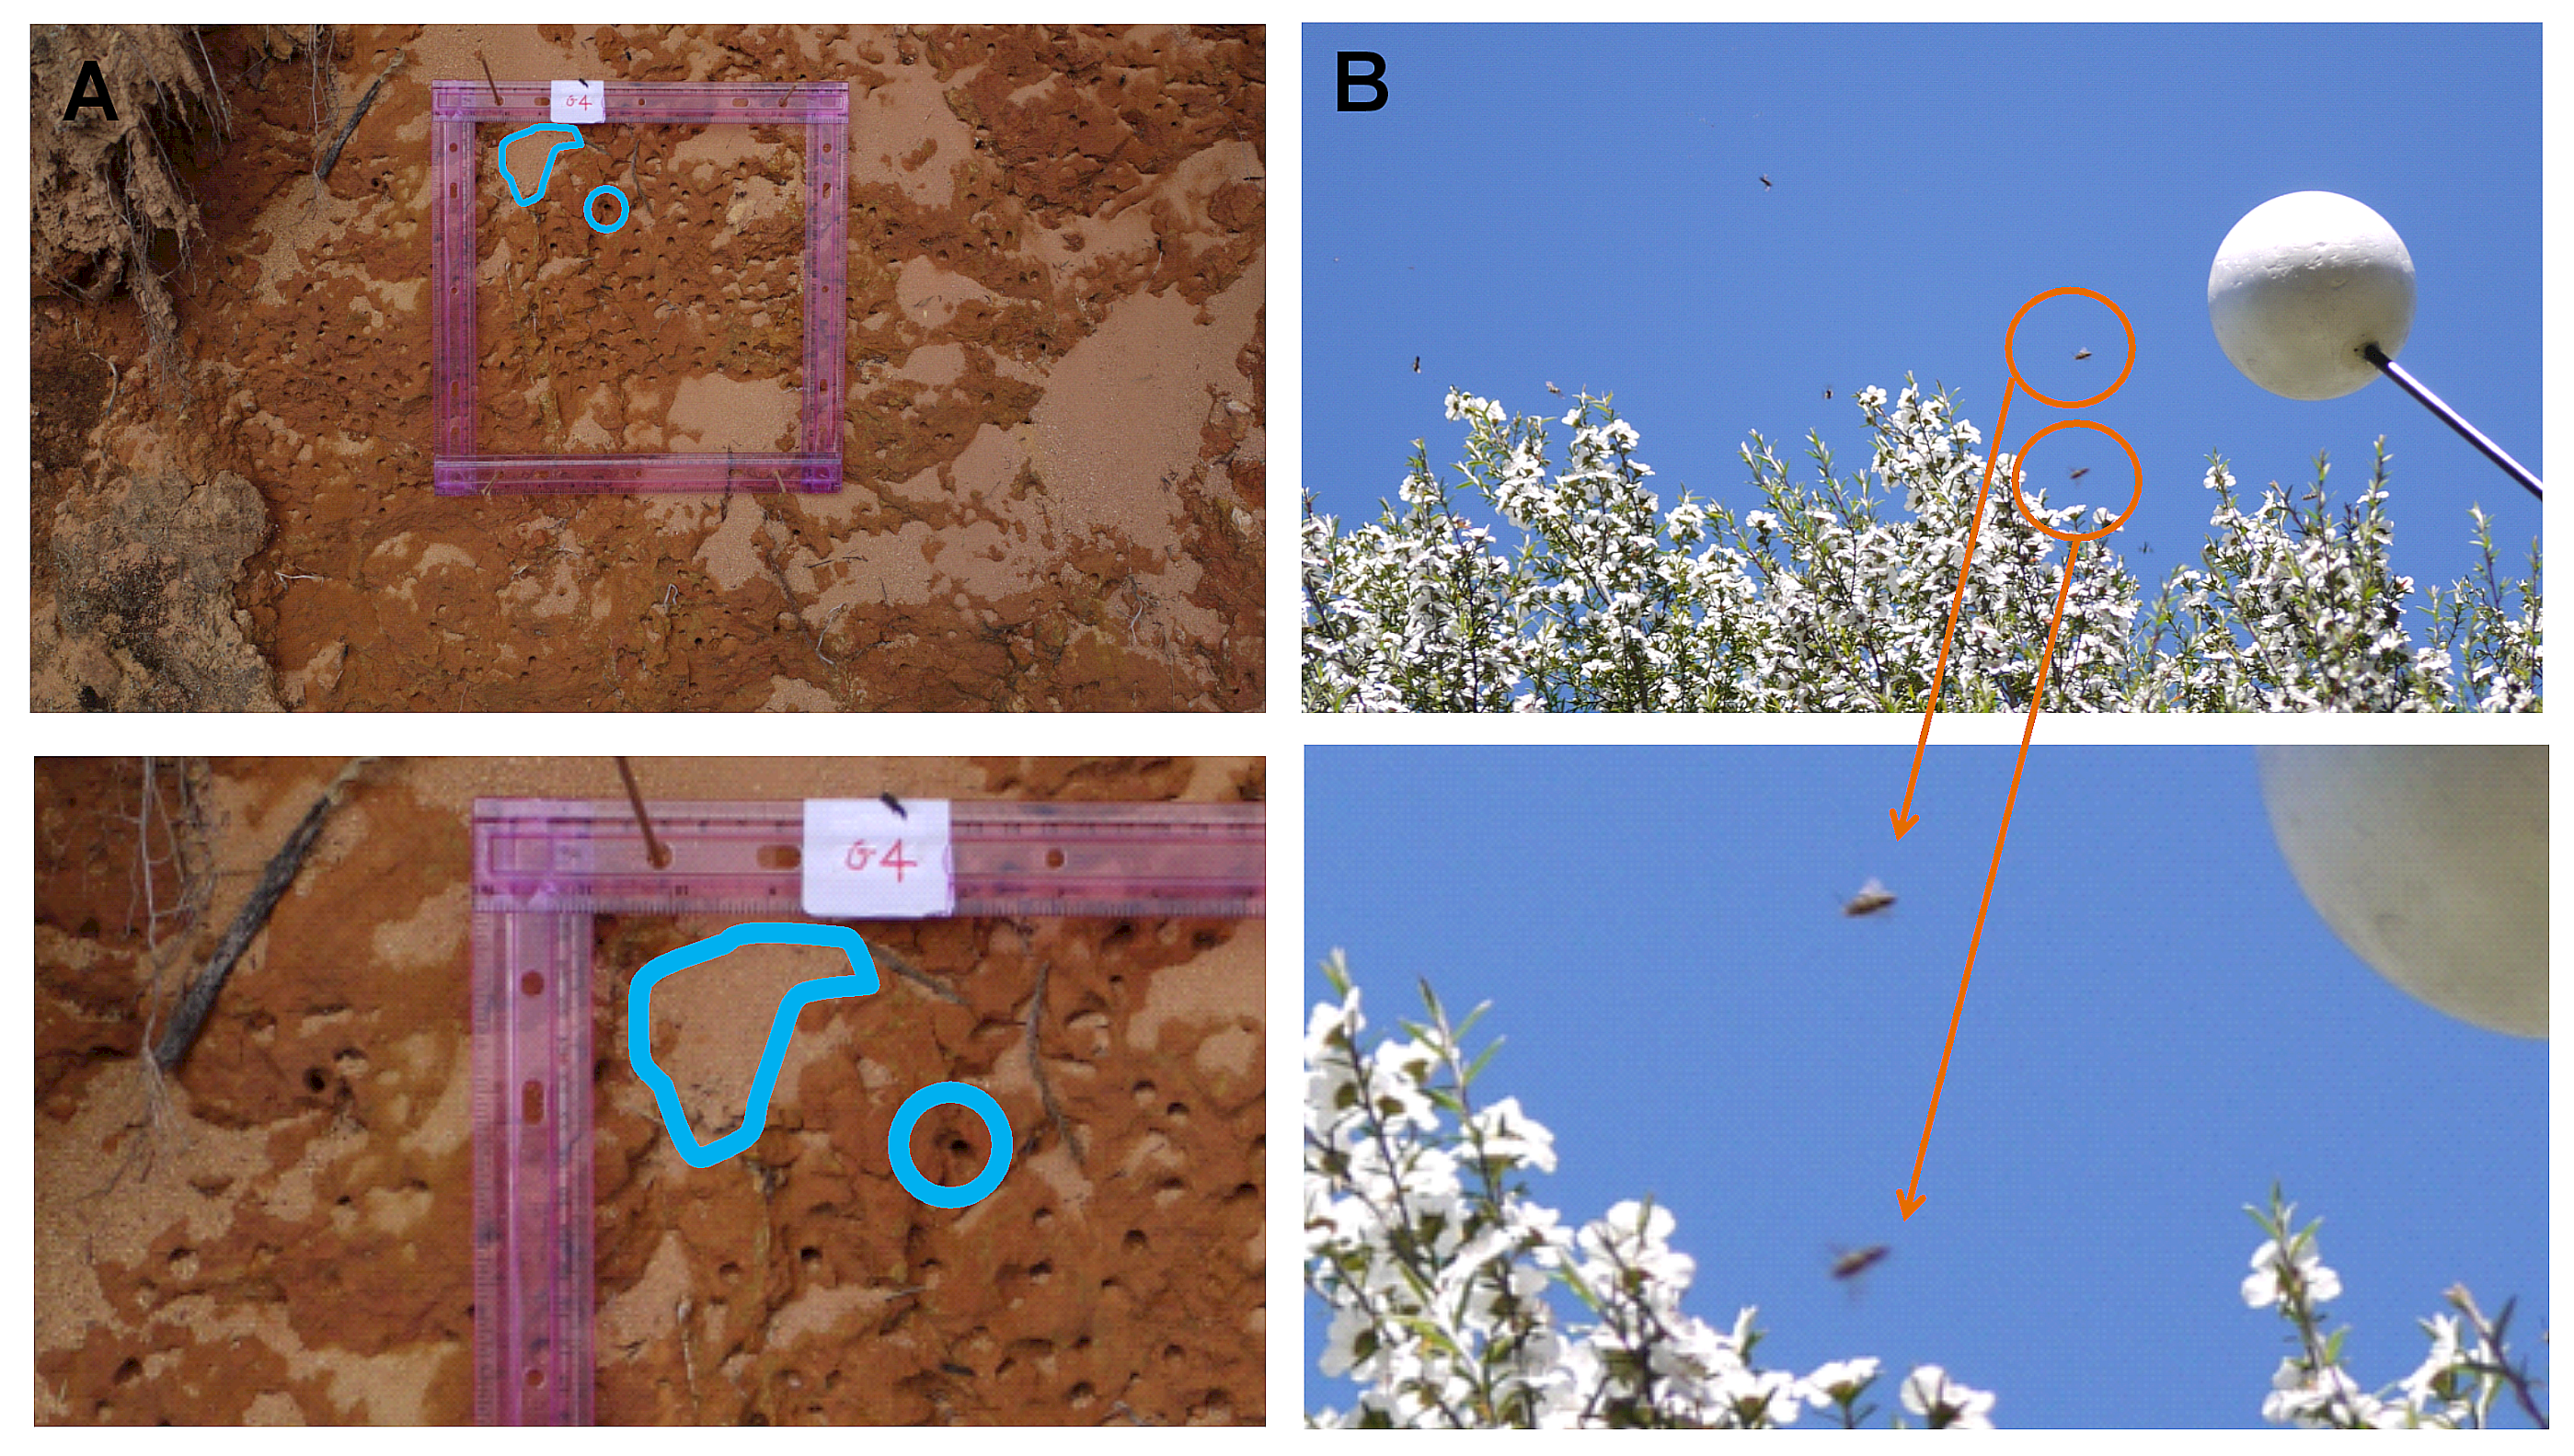
\includegraphics[width=1\linewidth]{gfx7/nests-flight/anif}} \\
\caption [Images of sweep net collections.]{Images of (a) sweep net collections and (b) standard of measures for monitoring -- grids for active nests (left) and a sphere for bees in flight (right).}\label{fig:measures-image}
\end{figure}

Finally, the field method for counting active nests were not overly complicated. Surveys were conducted each year around September. Monitoring was initiated when there was clear evidence the bees were emerging (e.g. either by signs of nest constructions or observations of bees in flight). At each monitoring location, the number of nests were counted using evidence of soil excavations or entry holes. The nest counts taken at the start of each season were important. The nest entry holes were more defined and easier  to count. Because of this they were the more reliable than counts taken towards the hight of the active flight season. Mid season the entry holes to active nests would become obscured by masses of soil from nest excavations. It was almost impossible to determine where the entry holes were in some cases. This was a particular issue at Mt. Tiger (Figure\ref{fig:wideclose-image}). The nesting community at Mt. Tiger was established along a roadside bank. Because of the structure and angle of the bank, the soil from nesting bees rapidly accumulated in some pockets and completely covered nest entrances. In contrast to Mt. Tiger, there were communities of bees established along a flat area of ground at Mt. Parihaka. These horizontal nests were much easier to count; at the start and throughout the season. This was because the mounds of white clay soil indicating nesting bees were easily separated from one another and from the ground surface vegetation as shown in Figure \ref{fig:signs-image}.

\section{Monitoring images}
Digital image formats and acquisition techniques are important aspects of an imaging system design. \marginpar{Image formats, quality and variability.}The decisions regarding the digital camera hardware and image format in this research were based on costs. An off-the-shelf \ac{DSLR} Panasonic DMC-G1 camera was used for acquisition of nest images which were saved in compressed JPEG format. Although off-the-shelf digital cameras and encrypted image formats are not recommended for biological image analysis they are used in some environmental image applications {ref}.

\subsection{Image format}
There are no agreed standards for raw files so proprietary platform dependent software is often bundled with off-the-shelf digital cameras to enable file processing. Silkypix\texttrademark~Software was bundled with the DLSR camera used in field monitoring. The software was platform dependent so use was restricted. Open-source software helped to mitigate proprietary format issues but with variable success. Raw files were not easily imported into Fiji or XnView. Reading and converting the RAW files was an added step in the image processing pipeline. During early tests the added file work was shown to be too resource intensive and time consuming to consider using raw files in the bee monitoring system. 

Nonetheless, the quality of image data can impact the reliability of image processing. At least where biological image analysis is concerned high resolution raw images are preferred. However, biological images are captured under laboratory conditions and memory capacity is not usually an issue. On-board camera memory was a consideration for field collections. Because the field camera had a limited amount of memory compressed high quality JPEG formats were more practical and cost effective. Some studies have shown image compression is not always an issue. Paola \& Schowengerdt \cite{Paola1995} for example, tested three different classification scenarios and found that high quality classifications could still be achieved with a \ac{CR} of 10:1 \cite{Paola1995}. 

The compression ratio of the field camera was closely examined to determine the qualitative affects on monitoring images. Since active bee nests are ill defined, a close-up image of an associated insect
the common New Zealand tiger beetle--\emph{Cicindela tuberculata} (Coleoptera: Carabidae) was used in the evaluations. The image was converted to a JPEG file with a CR of 34.71:1 using XnView software. After the image was compressed the affects were visually checked. The a close-up view highlights some minimal visible affects from the encryption. This can be seen in Figure \ref{fig:Image_quality} (a)--right as slight blocking. When images were converted on-camera the CR's were substantially lower at around 2.75:1. This level of compression was less than 10:1 and was well within the boundaries considered acceptable for image classification applications recommended by Paola \& Schowengerdt \cite{Paola1995} and others \cite{Lam2001, Zabala2011}.


\begin{figure}[!htbp]\myfloatalign
\includegraphics[width=0.9\linewidth]{gfx7/raw_tiffjpg}\\
\caption[Image quality and preparation for analysis.] {A raw image of a tiger beetle nest (background image) taken with the monitoring camera ( Panasonic) and a close-up example of file compression using XnView Software.} \label{fig:Image_quality}
\end{figure}

\subsection{Outdoor images}
A number of techniques can be used to help standardise image acquisition and reduce the affects of outdoor variations \cite{Burks2000}. Several techniques were tested during the prototyping stages of the monitoring system design. For example, flood lights were tested on monitoring nests to determine if the extra illumination would improve image quality. However, the challenges associated with outdoor imaging methods are fundamental constraints. They were not easily overcome in this research since field samples were necessary. Because the images of active nests were acquired outdoors they were variable and complex. It was not possible to control the quality of images. For example, the lighting conditions changed dramatically on cloudy days, sometimes within seconds. On windy days objects could be blown across the nest sites, and the field of view of the camera during image acquisition. This is common to many outdoor imaging applications as a review of current literature confirmed \cite{Burks2000,Feng2015a,Feng2015b}. There are few practical methods that can be used to improve the quality of natural outdoor images even though there are some novel approaches (e.g. see the design by Burks \cite{Burks2000}). A review of the current literature on this topic revealed  a number of studies that reported the problems associated with analysis of complex natural images could be mitigated by using \acp{RF} for image classifications \cite{Feng2015a,Feng2015b}. The studies showed there were good results from image segmentations using the \ac{RF} classifier even when compressed, outdoor images were acquired using off-the-shelf digital cameras \cite{Feng2015a,Feng2015b}. 

The quality of monitoring images was a key issue that had an critical impact on the design of the image-centric monitoring system. A closer examination of the nest images and the decisions that determined the imaging pipeline tools and methods are described in further detail throughout this Chapter.

\subsection{Examining nest images}
Biomedical imaging package \ac{Fiji} was the selected tool used for monitoring image analysis. The reasons for this have been mentioned previously. However, because Fiji is open source the methodology used throughout this thesis can be easily replicated. Fiji macro scripts are included in Appendices for reference and there are a range of resources for development of Fiji and ImageJ scripts available online.

Nest images were examined in Fiji. A test stack was compiled using representative nest images selected from each site-grid to reflect the range and variation typically encountered. The test stack, or a single slice from the stack were used to test a range of processing techniques examined over the next few Sections (\ref{fig:rep-nest-stack}).

\begin{figure}[!htbp]\myfloatalign
\includegraphics[width=1\linewidth]{gfx6/segtest/1rf}\\
\caption[Test stack of representative nest images]{Test stack of representative nest images in raw \ac{RGB} format. Slice 1 = Mt. Tiger (bank grid 1), slice 2 = Memorial Drive (bank grid 1), slice 3 = Mt. Parihaka (bank grid 1), slice 4 = Mt. Tiger (bank grid 2), slice 5 = Mt. Parihaka (horizontal ground grid 4), slice 6 = Mt. Tiger (bank grid 4)} \label{fig:rep-nest-stack}
\end{figure}

In most analysis workflows images are prepared by using \emph{contrast enhancement} or \emph{histogram equalisation} operations; generally called image normalisations. A single image of a horizontal ground nest was examined in \ac{Fiji} using different contrast enhancement settings to investigate the most appropriate levels for monitoring images. There were four different functions in the enhance contrast toolbox that were tested: 1) the percentage of \emph{saturated pixels}, 2) equalise histogram, 3) \emph{process all} and 4) stack equalise histogram. The test stack was processed using three different values of saturated pixels: 0.4\%, 40\% and 90\%. The results from tests are shown in Figure \ref{fig:fiji-menu} (b). 

The changes in contrast can be visually inspected in Figure \ref{fig:fiji-menu} (b). The third scheme was selected for pre-processing monitoring images; the number of saturated pixels was set to 0.4\%. This setting was useful for improving the visual qualities of the nest images for displaying on the \ac{LCD} monitor used in this research. Histogram equalisation was not used for nest images since this operation fundamentally changes the digital data.

\begin{figure}[!htbp]\myfloatalign
\subfloat[Contrast stretch on image slices]{\includegraphics[width=0.45\linewidth]{gfx7/thresh/mec}} \
\subfloat[\emph{Enhance contrast} pre-processing. ]{\includegraphics[width=0.45\linewidth]{gfx7/thresh/mscec}}
\caption[Fiji contrast enhancement.]{Image of a horizontal nest used to test the affects of (a) contrast stretching using 0.4\%, 40\% and 90\% saturated pixels (b) and Enhance contrast toolbox stack functions. Scheme 3 was used for all monitoring images. The number of saturated pixels was set to \emph{0.4\%} and the \emph{Process all slices} function was checked.}\label{fig:fiji-menu}
\end{figure}

\section{Segmentation methods}
Good segmentation techniques are those where, (1) pixels in the same category have similar values and form connected regions or (2) neighbouring pixels which are in different categories have dissimilar values. \marginpar{Segmentation challenges} The primary aim of all segmentation techniques is to quantify aspects of image data using reproducible and objective techniques, with some capacity to \emph{generalise} over a given range of image data variability. The performance of any segmentation method ultimately depends on the original image content and quality, the specific application constraints and characteristics, and the intended use of the information required to be extracted from images. 

To examine this further three segmentation techniques were tested on a sample of representative nest images. These included classical thresholding edge detection by Canny-Deriche filtering and statistical region merging.

\subsection{Thresholding by intensity}
Intensity based thresholding methods produce straightforward segmentations; they are simple, direct and easily programmed. If there are foreground objects or image features that are \emph{defined by intensity} then threshold procedures can outperform other methods. 

Suitable threshold levels were tested using slice 5 of the test stack (slice 5: site 2/horizontal ground nest/grid 4). Fiji Auto threshold {Try All}\footnote{Try All http://fiji.sc/Auto\_Threshold} \cite{AutoThresholdFiji} function was selected to determine which method best suited the nest image. The active nest in image slice 5, is visually noticeable; the white clay tumulus indicates at least one or two active nests. The intensity of soil means the image is relatively easy to make binary. The output stack results for automatic thresholds on slice 5 are shown in Figure \ref{fig:variability-tryall-threshold} below.

\begin{figure}[!htbp]\myfloatalign
\subfloat[Test slice 6: Mt. Parihaka ground nest image.]{\includegraphics[width=.45\linewidth]{gfx7/thresh/mgec5}} \
\subfloat[Test slice 1: Mt. Tiger roadside bank nest image.]{\includegraphics[width=.45\linewidth]{gfx7/thresh/tryall2}} \
\caption[Images of active nests and thresholding tests.]{Auto thresholds for monitoring images of (a) a horizontal ground nest (b) a roadside bank nest.}\label{fig:variability-tryall-threshold}
\end{figure}

The results demonstrate that from 16 possible schemes \emph{Minimum} returned the highest quality segmentation. In this case the image was adequately segmented \emph{before} any post-processing operations were applied. When post- processing operators were also applied the results confirmed an automatic threshold method using the \emph{Minimum} scheme would produce satisfactory image segmentations for horizontal ground nests. These are shown in Figure \ref {fig:threshold-six-post}(a)--(e). However, when the auto threshold {Try All} function was applied to test slice 1  the nest image was not properly segmented (slice 1: site 1/bank nest/grid 1). This is demonstrated in Figure \ref{fig:variability-tryall-threshold} (b). These results helped to define the constraints of segmentation methods. They showed the \emph{complete range} of monitoring images could not be segmented easily using intensity-based threshold levels. They also confirmed automatic thresholds could be used to segment images of horizontal grounds nests. Therefore they would be suitable for segmenting 1/6 {\scriptsize {th}} of the monitoring images collected.

\begin{figure}[!htbp] \myfloatalign
\subfloat[Binary output from six thresholding methods applied to the image of a horizontal ground nest (Mt. Parihaka, grid 4). Output slices 1-6 = Fiji Default threshold, Huang, Mean, MinError, Minimum and Otsu. ]{\includegraphics[width=1\linewidth]{gfx7/bin/1mt}} \\
\subfloat[\emph{Open} binary operation.]{\includegraphics[width=1\linewidth]{gfx7/bin/2mt}} \\
\subfloat[\emph{Fill holes} binary operation.]{\includegraphics[width=1\linewidth]{gfx7/bin/3mt}} \\
\subfloat[\emph{Close} binary operation.]{\includegraphics[width=1\linewidth]{gfx7/bin/4mt}} \\
\subfloat[\emph{Analyze particles} plugin: set to count all image objects between the sizes of 500-$\infty$ pixels with a circularity morphology between 0.1-0.9.]{\includegraphics[width=1\linewidth]{gfx7/bin/5mt}} \\
\caption[Six thresholding methods.]{Binary results from six thresholding methods (a) applied to a horizontal ground nest image. Common post-processing pipeline morphological operators were applied to the test image including (b) open, (c) fill holes, d) close and (e) count particles.}\label{fig:threshold-six-post}
\end{figure}

\subsection{Canny-Deriche filtering}\label{sec:canny-deriche-filtering-in-fiji}
Automatic thresholds work well when intensity is a feature that can be used to identify objects. This was demonstrated in the previous example. Sometimes there are other characteristics that can be used to define images such as the connected structures, outlines, areas or textural qualities of objects. Since it was not possible to use automatic thresholds on all monitoring images, two alternative methods for segmentation of active nests were tested. The first of these was an edge detection based thresholding method--\emph{Canny-Deriche filtering} \cite{Deriche1987}. 

Figure \ref{fig:segment-by-edge} demonstrates the affects of the Canny-Deriche filter after different smoothing factors ($\alpha$) were applied to the horizontal ground nest image. Six smoothing factors were applied to the ground nest image as follows: slices 1--6:  $\alpha = $ 1.0, 0.9, 0.7, 0.6, 0.45 and 0.15. The image results from each smoothing were compiled into a stack for visual inspection and comparison. The results from the edge-based thresholds indicated the method could be used to segment horizontal ground nest images. This is demonstrated in slices 1--6 on Figure \ref{fig:segment-by-edge} (a)--(f).

The lower smoothing values returned slightly better results, which can be seen from the final image segmentations in Figure \ref{fig:segment-by-edge} (e), slice 6. Overall however, edge detection did not provide any obvious additional benefits over the straightforward thresholds previously tested.

\begin{figure}[!htbp] \myfloatalign
\subfloat[Canny-Deriche filter results from different smoothing values slices 1-6: $\alpha=$ 1.0, 0.9, 0.7, 0.6, 0.45 and 0.15.]{\includegraphics[width=1\linewidth]{gfx7/edge/1me}} \\
\subfloat[Make \emph{Binary}.]{\includegraphics[width=1\linewidth]{gfx7/edge/2me}} \\
\subfloat[\emph{Open} binary operation.]{\includegraphics[width=1\linewidth]{gfx7/edge/3me}} \\
\subfloat[\emph{Fill holes} binary operation.]{\includegraphics[width=1\linewidth]{gfx7/edge/4me}} \\
\subfloat[\emph{Close} binary operation.]{\includegraphics[width=1\linewidth]{gfx7/edge/5me}} \\
\subfloat[\emph{Analyze particles} plugin: set to count all image objects between the sizes of 500-$\infty$ pixels with a circularity morphology between 0.1-0.9.]{\includegraphics[width=1\linewidth]{gfx7/edge/6me}} \\
\caption[Segmentation by edge detection.]{Segmentation by edge detection (a) applied to a horizontal ground nest image with a pipeline of common post-processing operations (b)--(f).\label{fig:segment-by-edge}}
\end{figure}

\subsection{Statistical region merging}\label{sec:statistical-region-merging-in-fiji}
In a final examination a region-based method, \ac{SRM} \cite{Nock2004, Nock2005} was tested on the ground nest test image. The results from \ac{SRM} investigations are shown in Figure \ref{fig:segment-by-region} (a)--(f) using six different values of $\emph{Q}$ (slices 1--6: $\emph{Q}=$ 1, 2, 3, 6, 8 and 16).

\begin{figure}[!htbp]\myfloatalign
\subfloat[SRM with slices 1--6 set to segment regions of $\emph{Q}=$ 1, 2, 3, 6, 8 and 16. ]{\includegraphics[width=1\linewidth]{gfx7/srm/1msrm}} \\
\subfloat[Make \emph{Binary}.]{\includegraphics[width=1\linewidth]{gfx7/srm/2msrm}} \\
\subfloat[\emph{Open} binary operation.]{\includegraphics[width=1\linewidth]{gfx7/srm/3msrm}} \\
\subfloat[\emph{Fill holes} binary operation.]{\includegraphics[width=1\linewidth]{gfx7/srm/4msrm}} \\
\subfloat[\emph{Close} binary operation.]{\includegraphics[width=1\linewidth]{gfx7/srm/5msrm}} \\
\subfloat[\emph{Analyze particles} plugin: set to count all image objects between the sizes of 100-$\infty$ pixels with a circularity morphology between 0.1-0.9.]{\includegraphics[width=1\linewidth]{gfx7/srm/6msrm}} \\
\caption[Segmentation by region merging.]{Segmentation by SRM (a) applied to a horizontal ground nest image with a pipeline of common post-processing operations (b)--(f).\label{fig:segment-by-region}}
\end{figure}

The method worked very well on test slice 5. Nonetheless, as was the case with the other methods tested, segmenting the range of monitoring images was a challenging. Ground truth labels--or manual annotations were added to the representative stack of nest images for comparison with binary results. Figure \ref{fig:threshold-variable-post} (a) confirms, most of the test images were over-segmented to degrees that could not be easily managed by post-processing operations. For example, there are no active nests in slice 1. Yet the Canny-Deriche edge detection and SRM methods produced binary outputs resulting in multiple segmentations. This is demonstrated in Figures \ref{fig:threshold-variable-post} (b)--(d) and  \ref{fig:threshold-variable-post} (e)--(g) respectively.

After applying post-processing operations a number of objects were detected that did not correspond to ground truth labels. In most analyses \emph{any} aspect of the imaging pipeline can be tweaked to accommodate image characteristics or to highlight the key data required for specific applications. However, there were \emph{no} techniques that could improve the variability of monitoring images and few image processing techniques that could improve image segmentations. It was concluded that neither of the techniques appropriately segmented the range of nest images. Because there was no single intensity value that could properly define the foreground active nests from backgrounds, none of the traditional methods were suitable for generalising over the range of monitoring images.

\begin{figure}[!htbp] \myfloatalign
\subfloat[Stack of representative nest images.]{\includegraphics[width=1\linewidth]{gfx7/annotate}} \\
\subfloat[The output from a Canny-Deriche filter on variable nest images with $\alpha=$ 0.15.]{\includegraphics[width=1\linewidth]{gfx7/edge/1meall}} \\
\subfloat[Make \emph{Binary}.]{\includegraphics[width=1\linewidth]{gfx7/edge/2meall}} \\
\subfloat[\emph{Analyze particles}.]{\includegraphics[width=1\linewidth]{gfx7/edge/6meall}} \\
\subfloat[The output from SRM on variable nest images with $\emph{Q}=$ 16.]{\includegraphics[width=1\linewidth]{gfx7/srm/1msrmall}} \\
\subfloat[Make \emph{Binary}.]{\includegraphics[width=1\linewidth]{gfx7/srm/2msrmall}} \\
\subfloat[\emph{Analyze particles}.]{\includegraphics[width=1\linewidth]{gfx7/srm/6msrmall}} \\
\caption[Tests on variable nest images.]{Stack of variable nest images (a) with ground truth annotations in blue. The binary results from the (b) Canny-Deriche filter edge detection and (e) SRM and final post-processing operations.\label{fig:threshold-variable-post}}
\end{figure}

\section{Trainable segmentations} 
There were other characteristics in the monitoring images that defined active nests; such as colour and texture of tumulii. Overall the monitoring images were highly variable across time and space; therefore image segmentations were challenging. The images of horizontal nests would be adequately segmented by other methods. In the previous tests \ac{SRM} performed well; it was easy to apply and produced a properly segmented image of the horizontal ground nest. However, few if any of the other image types were properly segmented. At least not to the degree necessary to have confidence in the results from post-processed binary operations. Therefore although \ac{SRM} worked well on images of horizontal ground nests, the method would not have performed well on the other 83\% of monitoring images collected. 

A review of current literature showed that when other segmentation methods fail machine learning could provide a plethora of alternative solutions. Some of these were tested on the stack of representative nest images using Fiji and the \ac{TWS} toolbox. As a consequence {semi-supervised} machine learning tools were considered the \emph{only valid option} for nest image segmentations. The remaining Sections are therefore dedicated to \acf{TWS}. This includes an over-view of training methods and optimisation techniques and a review of the classifiers designed for the image-centric monitoring system. 

Trainable image segmentation techniques work by utilising human visual knowledge to provide a machine learning algorithm with a set of {expertly labelled examples}. In \ac{TWS} a user provides two sets of example labels; \ac{ROI} tools are used to select traces of pixels belonging to foreground (class 1) and background (class 2) objects. A range of filters are applied to original image data. These are used to create a separate features stack. A user may select any combination of filters from a possible twenty. These can be grouped according to their main filter functions (Table \ref{tab:tws-features}). During the learning process a Weka machine  algorithm uses the examples provided, and the features stack to construct a classifier. The classifier can be used to segment similar types of images, including the one it was trained on. This is a summary of the overall the process but it is relatively straightforward.

There are some aspects of trainable segmentations that are difficult to quantify. For example, it can be hard to determine what combination of image features best describes key objects. Consequently, some aspects of classifier training are intuitive and subjective. There are also other confounding decisions to consider before applying machine learning for image segmentations, which will be discussed further. However, providing a user selects appropriate representative pixel samples and chooses filters that will provide a rich features stack for the analysis, machine learning algorithms work very well. They can surpass other methods especially on challenging image segmentations and preliminary tests on the stack of representative nest images confirmed their effectiveness.

A classifier was constructed using \ac{TWS} to segment the stack of representative stack of images. The results from the classifications were a stack of binary images which are shown in Figure \ref{fig:segment-by-rf-all}. The machine learner classified every pixel in the test images as belonging class 1 or 2. The classifier adequately segmented all the slices of the nest images where the previous methods were inadequate. This is further demonstrated by comparing the test images in Figure \ref{fig:threshold-variable-post} with the classified output from a machine learner in Figure \ref{fig:segment-by-rf-all}. When the variable image stack was used for comparative checks the final number of nest counted from the machine learning method, shown in Figure \ref{fig:segment-by-rf-all} (g), was in much closer agreement with those visually counted and annotated on images (i.e. ground \emph{truth labels}), shown in Figure \ref{fig:segment-by-rf-all} (a). The segmentation results on the variable nest images were \emph{significantly} different to those produced by classical Canny-Deriche edge detection and SRM techniques (Figure \ref{fig:threshold-variable-post}). The difference between the methods was more obvious when the final particle count results from all methods were visualised alongside each other; these are shown in Figure \ref{fig:segment-finalcounts_all}.

\begin{figure}[!htbp] \myfloatalign
\subfloat[Annotated stack of representative nest images.]{\includegraphics[width=1\linewidth]{gfx7/annotate}} \\
\subfloat[Classificed output from TWS.]{\includegraphics[width=1\linewidth]{gfx7/rf/1mrf}} \\
\subfloat[Make \emph{Binary}]{\includegraphics[width=1\linewidth]{gfx7/rf/2mrf}} \\
\subfloat[\emph{Open} binary operation.]{\includegraphics[width=1\linewidth]{gfx7/rf/3mrf}} \\
\subfloat[\emph{Fill holes} binary operation.]{\includegraphics[width=1\linewidth]{gfx7/rf/4mrf}} \\
\subfloat[\emph{Close} binary operation.]{\includegraphics[width=1\linewidth]{gfx7/rf/5mrf}} \\
\subfloat[\emph{Analyze particles} plugin: set to count all image objects between the sizes of 100-$\infty$ pixels  with a circularity morphology between 0.1-0.9.]{\includegraphics[width=1\linewidth]{gfx7/rf/6mrf}} \\
\caption[Trainable segmentations on variable nest images.]{Trainable segmentations on variable nest images (a) with ground truth annotations in blue with a pipeline of common post-processing operations (b)--(g).\label{fig:segment-by-rf-all}}
\end{figure}

\begin{figure}[!htbp] \myfloatalign
\subfloat[Ground truth labels on the stack of representative nest images.]{\includegraphics[width=1\linewidth]{gfx7/annotate}} \\
\subfloat[Canny-Deriche edge final results.]{\includegraphics[width=1\linewidth]{gfx7/edge/6meall}} \\
\subfloat[\ac{SRM} final results.]{\includegraphics[width=1\linewidth]{gfx7/srm/6msrmall}} \\
\subfloat[\ac{TWS} final results.]{\includegraphics[width=1\linewidth]{gfx7/rf/6mrf}} \\
\caption[Comparison of segmentation methods.]{The ground truth labels of the (a) stack of variable nest images are compared to the final post-processed outputs from segmentations using the: (b) Canny-Deriche edge detector, (c) \ac{SRM} and (d) \acp{TWS}. Results from \acp{TWS} are in closer agreement with the ground truth labels in each slice.}\label{fig:segment-finalcounts_all}
\end{figure}

\begin{table}[!htbp]\myfloatalign \caption[Trainable  Weka Segmentation filters.]{Filters available in the TWS plugin grouped by type.}\label{tab:tws-features} 
\begin{tabular}{lp{3.0in}}\toprule
\emph{Edge detectors.} & Indicate boundaries: Laplacian, Sobel, difference of Gaussians, Hessian matrix eigenvalues and Gabor filters. \\
\emph{Texture filters.} & Extract textural information: Minimum, maximum, median, mean, variance, entropy, structure tensor. \\
\emph{Noise reduction filters.} & Smooth images: Gaussian blur, bilateral filter, Anisotropic diffusion, Kuwahara and Lipschitz. \\
\emph{Membrane detectors.} & Localised membrane-like structures of a certain size and thickness. \\ \bottomrule
\end{tabular}
\end{table}

\clearpage

\section{Empirical lessons}
Since 2010 the \ac{TWS} workbench has undergone significant developments. \marginpar{\ac{TWS} experiments, rules-of-thumb and optimal parameters for classifiers.} Each year the package has become more versatile. For example, early tests and initial training investigations could only be performed on 8-bit grey-scale images and \acs{TWS} was not initially integrated with Weka \cite{Hall2009}. Also, \acs{RF} \emph{feature importances} were not easily examined during early tests, however for the final analysis it was possible to compute feature importances and quantitatively examine the impact of filters on classifications. For this reason over the course of this research, each successive classifier testing training and analysis changed \cite{Hart2007}. The methods used for nest classifications have steadily improved. The following sections discuss the final results from base-classifier investigations; tuning options and training methods.

\subsection{Concepts important for classifier training}
The performance of the final monitoring classifiers was dependent on the quality of classifier training. This included the images selected for training, the traces supplied to represent classes during training and the filters used to construct the features stack which were provided to the \ac{RF} algorithm for training. Some of the important questions considered were:

\begin{enumerate}
\item How well do the training images represent the monitoring  images? 
\item Which pixel traces best contribute towards classifier learning? 
\item What image features best help to describe active nests?
\item Can the key features of active nests be enhanced?
\end{enumerate}

In order to determine the optimal parameters for \acp{TWS} and the \ac{RF} classifier, small repetitive tests were applied to the stack of representative nest images. There were to main aspects to consider. The first was to determine which features were the most important for nest-classifications. This process is referred to as feature engineering. The second was to determine the best tuning settings for the \ac{RF} model; generally referred to as classifier optimisation. These are discussed in the next sections.

\subsection{Feature engineering for nest classifiers}\label{sec:feature-engineering-for-nest-classifiers}
Feature engineering was one of the more difficult processes to evaluate. This was because it is the \emph{total combination} of features that contributes to the final accuracy of machine learning models; according to most current literature. Generally, the more features that are provided during training, the better the final classifiers are. However, there were computational costs associated with the construction of the features stacks for monitoring nest-classifiers. Stack creation and processing, was fundamentally limited by the amount of desktop RAM available; this was around 7.2Gb in total. 

Therefore it was important to examine the affects of removing \emph{seemingly} irrelevant features and replacing them with the most \emph{obviously} relevant ones. Textural and noise reduction filters were considered the most appropriate for describing active nest objects in the monitoring images. It was hypothesised that these filters would also be the most important for classifying images of active nests.

Initial tests were performed and the classifiers were re-tuned based on:

\begin{itemize}
\item The feature importances output during training.
\item The total processing times -- the time to construct features stack, time to train the classifier and time to complete classifications.
\item The classified binary image results -- fully post-processed for comparison against ground truth labels.
\item The out of bag error during training.
\end{itemize}

The filters that did not obviously or significantly contribute to the accuracy of final classifiers were removed and the training was re-run. The segmentation results were checked by comparing post-processed binary nest counts against raw \ac{RGB} monitoring images and manual-field nest counts. This process was repeated until the images from each representative slice were sufficiently segmented.

During the first test, classifier C1 was set to default parameters. Of the 79 filters around 46 ($58\%$) did not provide any additional information. Therefore the second test classifier, C2 was tuned for to provide the optimal nest image features. Similarly, at least half of the feature data provided to C2 did not obviously contribute to the final classifications. Furthermore the time taken to construct the features stack increased due to the iterative process from the Anisotropic diffusion filter. 

The out of bag error was lower for test classifier C2, but at the expense of increased processing resources and time. Therefore classifier C3 was tuned to optimise the speed of feature stack creation, classifier training, construction and application. Only the most important textural filters were selected. The final evaluations were good; they showed all the features provided for the training of classifier C3 were important for classifications.

\subsection{Calibrating random forest models}\label{sec:calibrating-random-forest-models}
Generally there are no classifier performance penalties for having a \ac{RF} with more trees since this normally reduces the out of bag error and increases the number of correctly classified pixels. However, as described in the previous section, there were \emph{resource} issues to consider since training and classifications would have taken longer. Also, according to Breiman \cite{Breiman2001} the number of trees in a \ac{RF} should be set to 200 initially and tuned as required. While the initial number of random features for \ac{RF} is given by the square root of the maximum number of features \cite{Breiman2001}. In the final feature-speed optimised test there were 20 features used to construct the test classifier, C3. Thus following Breiman's \cite{Breiman2001} rule of thumb the ideal number of random features provided to the model for training should have been around 5. These two parameters were evaluated with Weka Experimenter using the approximate guidelines suggested by Breiman \cite{Breiman2001}.

In the fist analysis, twenty one \ac{RF} models were loaded into Weka Experimenter {Algorithms} for testing and the experiment was saved for repeat investigations. A 10 fold cross validation with a maximum of 10 iterations were selected for tests and used in the analysis. Each classifier model was tuned with a different number of trees. These were set between $ N=10 - 1000 $. The out of bag error and overall time to complete processing was evaluated. The results showed the processing time exponentially increased as the number of trees increased. The tests also indicated there is was little improvement in the out of bag error beyond a certain number of trees. For example, the gains were not significant after $N = 150$. Therefore on the balance between processing time, resource usage and error reduction, the total number of trees for the test classifier C4 was set at $N = 50$. The test classifier C4 was re-run via \ac{TWS}. The total model processing was around 11 x faster than C1; 30 x faster than C2 and 2 x faster than C3 therefore a considerable improvement in processing time was achieved by optimising the features and number of trees.

In the second analysis, twenty \ac{RF} models were added to Weka Experimenter Algorithms for testing using a 10 fold cross validation experiment with 10 iterations. Each classifier model was tuned with a different number of random features. These were set between $M = 0 - 20$. The test results indicated the classifier performance \emph{improved} when more \emph{random features} were provided to the model for training. These evaluations also confirmed of Breimans \cite{Breiman2001} rule of thumb for selecting the ideal number of random features. For example at $M = 8$ the $oo_b =  0.62\%$ which was slightly better than out of bag error returned for classifier C4 $oo_b = 1.083\%$. These improvements were gained at little processing expense. Therefore the final monitoring classifiers were constructed with $N = 50$ and $M = 8$. 

\subsection{Benchmarking classifier performances}
The previous investigations confirmed the ideal features that should be provided to the monitoring classifiers for training; and the ideal tuning parameters for the \ac{RF} models. \marginpar{Determining which were the most important performance measures.} However, although \ac{RF} model is the default machine learner in \ac{TWS}, there are up to fifty different types of Weka machine learners available. In theory, other types could have been selected and trained to classify the monitoring images. For example, support vector machines are popular classifiers. They also perform well in some applications and are generally believed to be one of the most accurate classifiers available to date.

Therefore, in order to verify the performance of the \ac{RF} models, the final test classifier, CF ($ N = 50 $, $ M = 8 $), was compared to other well known machine learners using Weka Experimenter. The purpose of these tests were to asses the performance of the \ac{RF} models over other types of machine learners when applied to the data-set created from the representative stack of nest images. A 10 fold cross validation method, with a maximum of 10 iterations were selected for tests. Four \ac{RF} models were added to the experiment including the final monitoring classifier which was the benchmark model. Six other models were included and are listed below. All other classifiers were left at Weka or Fiji default settings. The percentage of correctly classified instances were reported for the analysis using $n = 1000$ data results; with a confidence of 0.05 in a paired-corrected two tailed test.

Benchmark results showed there were no signifiant improvements by any other models over CF. Three gave results that were statistically worse. The naive Bayes model (M8) did not perform as well as classifier CF on the test data-set. Correctly classified instances were lower at $90.63\%$. Unexpectedly naive Bayes results were lower than the ZeroR (M2) model which was the baseline classifier and was expected to give the lowest benchmark; it returned a result of $90.35\%$. The VotedPerceptron (M9) and SMO (M10) models returned a lower number of correctly classified instances compared to CF; $95\% $ and $96.72\%$ respectively. The results are listed below, including a brief description of the model, the percentage correctly classified instances and the Weka model ID indicating the number of tuning parameters associated with each classifier.

\begin{enumerate}
\item [M1] Final monitoring classifier (CF)--99.42\%.\\hr.irb.fastRandomForest.FastRandomForest-I|50|-K|8|-S|1
\item [M2] Baseline model--94.88\%\textasteriskcentered \\rules.ZeroR 
\item [M3] Weka Decision Tree--98.37\%\\trees.J48-C 0.25 -M|2 
\item [M4] Weka Random Tree--98.02\% \\trees.RandomTree-K|0|-M|1.0|-V|0.0010|-S|1 
\item [M5] Weka Random Forest--99.19\% \\trees.RandomForest-I|10|-K|0|-S|1|-num-slots|1 
\item [M6] \ac{TWS} Fast Random Forest--98.95\% \\ hr.irb.fastRandomForest.FastRandomForest-I|50|-K|2|-S|1 
\item [M7] \ac{TWS} Fast Random Forest--99.07\% \\hr.irb.fastRandomForest.FastRandomForest-I|200|-K|2|-S|1
\item [M8] Weka Naive Bayes--90.35\%\textasteriskcentered \\bayes.NaiveBayes 
\item [M9] Weka Neural Network--95.71\%\textasteriskcentered \\functions.VotedPerceptron-I|1|-E 1.0|-S|1|-M|10000
\item [M10] Weka Support Vector Machine--96.74\%\textasteriskcentered \\functions.SMO-C|1.0|-L|0.0010|-P|1.0E-12|-N|0|-V|-1|-W|1|-K|\\
functions.supportVector.PolyKernel-E|1.0|-C|250007 
\end{enumerate}

The test results probably could not be used to \emph{preclude} the usefulness of other classifiers for the nest-image segmentations. However, the results did highlight the difficulties associated with calibrating some models. Extensive skills and time are required to tune specific machine learners for any given task; and most require tuning for each specific task. In the benchmark tests only two of the \ac{RF} models were tuned, the C4 and CF test classifiers.  The other models were left at \ac{Fiji} or \ac{Weka} default settings. This was because most were too complex to attempt tuning. As previously mentioned, Weka has at least fifty different types of models. Each model requires specific tuning and the number of optimisation parameters varies between classifiers. The tuning options for each algorithm can be identified from the Weka model  names. For example, the VotedPerceptron (M9) has 8 tuning parameters and the SMO (M10) has 16. The complexity of the optimisation task for each model increases with each added parameter. Therefore no final conclusions were reached about the performance of one type of classifier, over another type. 

The overall objectives of the image-centric monitoring systems were equally important to consider. At least one of the aims of this research was to present a \emph{practical} image-centric monitoring method for native bees. Ideally by selecting the most appropriate tools currently available (during each stage of the imaging pipeline) so they could be used in the most efficient way possible and easily replicated. However, there were no major constraints regarding the types of tools designated for the imaging system. Therefore the benchmark tests confirmed two central ideas:

\begin{enumerate}
\item It was more productive to concentrate on tuning a single machine learner very well, using fully documented methods, rather than comparing the performance of different algorithms.
\item On the nest-image segmentation task, and in comparison to other Weka models, the \ac{RF} classifier was easy to tune, train and apply.
\end{enumerate}

Because image classification tools were a key aspect of the image-centric monitoring system at the segmentation stage of the imaging pipeline, it was apparent the entire training process would need to be easily replicated by others. It is possible other algorithms could have outperformed the \ac{RF}. However, without a good knowledge of the affects of tuning parameters the optimisation of other models was considerably more complex. In comparison to some Weka algorithms, the \ac{RF} classifier was straightforward to tune and easy to train. When it was applied to the stack of representative nest images the segmentations results were sufficient. For these reasons the \ac{RF} classifier was selected for monitoring image segmentations. The remaining discussions therefore concentrate on the \ac{RF} classifier as it was applied to segment images of active nests.

\subsection{Segmentation performance}
The importance of manual and visual agreements for active nest counts.\\
In biomedical imaging applications, segmentation metrics are generally applied to measure the performance of techniques of methods. \marginpar{Manaul nest counts and visual image-count agreements.} This is because microscopic images are normally central in most analyses. In these applications, the most common benchmarking method is to provide manually annotated ground truth labels for final comparisons. There are few other avenues that can be used to determine the validity of automated image segmentations in these cases. However, in this research, the number of active nests that are represented in each of the monitoring images was manually counted in the field. Therefore the manual-field nest counts provided a valid benchmark for comparison. It was not necessary to evaluate the image-centric monitoring system results in terms of the segmentation metrics. Even though manual-image nest counts were also recorded, the agreements between manual-field and automated counts were more critical in the final analyses. Nevertheless, visual analyses of nest image segmentations was a necessary part of the development of the image-centric monitoring system. Image segmentations were constantly checked and used to optimise classifiers and refine post-processing operations. These methods are discussed in the following paragraphs.

The representative image stack of six images were fully processed using the final test classifier CF and the results were visually assessed. Original training for the test classifiers was completed in a single session. This was not sufficient to properly train the classifier. When the segmentations from CF were post-processed, the final nest counts did not correspond well with either the manual image or field counts for the representative stack of images. The number of objects counted in slice 6 was particularly high at 64 (Table \ref{tab:Cf-counts}). Therefore a single trace was added and the model was trained again (CF2). The segmentation results were checked; another trace was added and the model was trained a final time (CF3). 

The final counts were visually checked against raw \ac{RGB} images for verification and against the manual field counts. This is summarised in \ref{tab:Cf-counts} below. The output log from \ac{TWS} training is shown in Listing \ref{cd:cf-retrain-output}. 

\begin{table}[!htbp]\myfloatalign \caption[Final count results from test classifier CF.]{The final automatic count results on representative images (slices s1--s6) using CF$ _{rt} $ compared to manual-image and manual-field counts.}\label{tab:Cf-counts} 
\begin{tabular}{lllllll} \toprule
Method &	s1 &	s2 &	s3 &	s4 &	s5 &	s6 \\\toprule
CF1 &	21 &	11 &	14 &	22 &	4 & 64 \\
CF2 &	21 &	2 &	3 &	13 &	3 & 14 \\
CF3 &	7 &	1 &	8 &	4 &	2 &	3  \\
Manual image &	3 &	3 &	3 &	2 &	2 &	2  \\
Manual field &	2 &	4 &	4 &	3 &	4 &	9  \\
\bottomrule
\end{tabular}
\end{table}


\begin{lstlisting}[float, language=java, caption={[Fiji output log from test classifier.]Fiji output log from test classifier (CF) re-training.}, label=cd:cf-retrain-output]
----------------------------
CF1 Training input:
# of pixels selected as class 1: 44
# of pixels selected as class 2: 816
Creating training data took: 38ms
Training classifier...
FastRandomForest of 50 trees, each constructed while considering 8 random features.
Out of bag error: 0.581%
----------------------------
CF2 Training input:
# of pixels selected as class 1: 44
# of pixels selected as class 2: 864
Creating training data took: 34ms
Training classifier...
FastRandomForest of 50 trees, each constructed while considering 8 random features.
Out of bag error: 0.661%
----------------------------
CF3 Training input:
# of pixels selected as class 1: 44
# of pixels selected as class 2: 996
Creating training data took: 28ms 
Training classifier...
FastRandomForest of 50 trees, each constructed while considering 8 random features.
Out of bag error: 0.577%
\end{lstlisting}

The number of pixels representing active nests (class 1) was not altered for classifier CF re-training; the number of background pixels (class 2) for CF--class 2 = 816, CF2--class 2 =  864 and C3--class 2 =  996. Output results also showed there was little change in the out of bag error between classifiers: CF1--$ oo_{b} = 0.581\%$, CF2--$ oo_{b} = 0.661\%$ and CF3--$ oo_{b} =0.577\%$. However, the segmentations changed markedly.

The number of objects counted in slice 1 and 8 were marginally raised. All other slices were reasonably well segmented. These results highlighted several concepts.  Firstly, the classifiers could be retrained using a very minimal number of corrective-traces. Secondly, for nest images these corrections were always traces of background pixels (e.g. class 2). Thirdly, it was difficult to train the test classifiers to properly segment all the slices in the representative stack (e.g. slice 1 and 8). Finally, the out of bag error could not be relied on to reflect the quality of image segmentations.

\subsection{Summary of classifier tests}
The lessons gained from empirical analysis and test classifier performance tests contributed greatly to the training methods adopted for monitoring images. There are no standard procedures that can be applied. Each machine learning model is tuned to perform well on a specific task. Also, there are hundreds of automatic and semi-automatic segmentation algorithms that have been developed since the advent of digital images. No single method could be considered appropriate for all types of images. Those designed for a particular type of image are not always applicable to others. In this research the \ac{RF} was selected and tests confirmed they are easy to train, tune and apply.

The variability of active nest images presents a challenge for \emph{any} classification model. Monitoring photographs were inconsistent and diverse. The same active nest monitored over time could change in colour and texture as the local landscapes naturally altered. The nests of native bees were variable at coarse and fine scales. Nests within the same community could be vastly different. They also varied between geographically separated communities as natural landscapes changed.

Therefore in order to gain the best possible performance of the \ac{RF} classifier for this analysis \emph{and} so training could be \emph{closely replicated} by others, some general rules for training were adopted. The term closely replicated comes with a caveat. The semi-supervised training method cannot actually be repeated, since each time a classifier is trained the final model will always be different. When a new model is applied to the same dataset it will produce alternative segmentation results. \ac{RF} models are also constructed with a random seed which is used during training. Because the processes are stochastic, the random seeds, models and trace data-sets would be necessary in order to reproduce the same image segmentations.

The tests highlighted both the strength and weakness of semi--supervised machine learning. User-supervised learning \emph{can improve} image classifications because humans draw on considerably more knowledge when performing manual
segmentations. But a human-interactive approach is dynamic. Therefore the performance of final classifier models are dependent on a number of subjective choices. Such as the images used for training, the human-selected traces provided during training and the suitability of features supplied to the classifier during construction. As mentioned previously, feature engineering can be ill-defined. Although the importances of single features can be analysed, it is the combined value of all features that contribute to final model performances. The interaction between training features cannot be fully analysed since the process is dynamic and it occurs during classifier training.

Nevertheless, and despite these considerations, on the task of segmenting active nest images there were few other image analysis options that could perform appropriately with the monitoring images. As demonstrated, most traditional methods cannot be used to segment the range of nest images gathered during field monitoring. Some could be used to segment horizontal grounds nest images since they are much easier threshold. Statistical region merging performed well segmenting images of horizontal nests. However most traditional methods, which are based only on the intensity information of pixels, are not suitable for segmenting the range of variable nest images. 

The \ac{TWS} tests also demonstrated the tools and methods to test, train and apply machine algorithms are freely available in software platforms such as \ac{TWS} and \ac{Weka}. \ac{TWS} is designed to use human knowledge in the segmentation process to improve the accuracy of the labelled regions. The algorithms in \ac{TWS} have been developed for natural and medical images but they can easily be applied to other tasks. Classifiers such as the \ac{RF} can be adapted for other types of images, in different applications using the \ac{TWS} platform. The software is easy to work with and is accessible to experienced and inexperienced users. The methods used to train \ac{RF} classifiers for segmenting the nest-monitoring images, using \ac{TWS} are discussed in the next Section. 

\section{Monitoring classifiers}
Typically the more trees and features that are used to train \ac{RF} classifiers, the better the final image segmentations are. However the computational costs increase as the number of features and trees grow \cite{Latinne2001}. This was an important consideration. Computer hardware and performance limited the final design of monitoring classifiers. For this reason, a minimalistic approach was adopted. Classifiers were optimised for speed to reduce the overall time required to process the monitoring images. A total of 1896 slices were processed, each image was 32-bit RGB, 500 x 500 pixels in size. Final classifications were completed in a day, substantially improving on previous analyses \cite{Hart2004,Hart2007,Hart2011,Hart2012,Hart2014}. Additionally, any obvious processing errors could be quickly rectified and the batch classifications re-run.

\subsection{Variability of training images}\label{sec:training-stacks}
Four training stacks were collated for each site. To simplify and speed up the training process each site-grid classifier was trained separately using respective stacks. This method also improved overall classifications since models could be constructed on a sub-sample of variable images and tuned for the specific image types associated with each monitoring site. There were twelve stacks in total, four per site.

\subsection{Morphological operators tuned for segmentations}\label{sec:post-processing}
Before the final post-processing operations were applied to the classified stack of monitoring images, several morphological operations and pipeline combinations were empirically tested using the small test stack. When the morphological operations were completed the counted results were visually checked against the original \ac{RGB} monitoring images and against the manual field counts.
It is important to point out, the post-processing operations were tuned specifically for the segmented monitoring-images that were produced using the CF classifiers. If new classifiers were constructed, new post-processing operators would most likely be necessary. This is because even if the same method is used to construct the nest-classifiers, the final models would not be exactly the same. Thus they would not produce replica image segmentations.
Additionally, the performance of final classifier segmentations were compared to nest-segmentations produced using classical methods. But, there was no attempt to tune the post-processing operators for image-segmentations that were produced from the classical intensity-based methods. It is possible, although very unlikely, the final nest count results from the classical methods could have been improved by morphological operators.

\section{Verification methodology}\label{sec:verification}
As discussed previously, classifier performance evaluations provided confirmation of suitability of the \ac{RF} as machine-learning tool for nest image segmentation. When combined with the functionality the \ac{TWS} workbench, they were easy to train, test and apply. Segmentation of nest images using the model were good enough given the irregularity of image data; and they were considerably better than the classical methods tested. When the \ac{RF} was compared against other machine-learners, classifier tests and benchmark analysis did not necessarily preclude the suitability of other models. But, there were practical benefits associated with the \ac{RF} classifier that could not be underestimated. These benefits probably account for the popularly of \acp{RF} in real-world data applications and they contributed to the adoption of the model for nest image-segmentations.

However, the main verification of the image--centric monitoring method primarily focused on the agreements between manual--field and automatic nest counts. Secondary to this were the differences between manual-image counts compared to the automatic and manual-field counts. Inter-observer correlations between manual-image counts were also measured. There were insufficient data for inter-observer correlations between the manual-field counts by two observers since field data were collected primarily by a single observer. Before the final comparisons were made, the automatic nest count results were modified. The reasons for this are outlined further in the proceeding paragraphs.

\subsection{Replica image collections?}
Each image collection was comprised of near-replica images. They were data collected from the same location, grid and day but separated by minutes:seconds. Separate collections were therefore comprised of different images; each single one was acquired under varying natural conditions. During preliminary analysis, there were some individual nest counts that were vastly different between the collections. This was unexpected. The reasons for the variations were investigated further. Where count data was significantly different between the collections, the raw monitoring images were visually checked. A pdf document  comprising of raw \ac{RGB} monitoring images alongside the count overlay results, were used to visually investigate discrepancies. It was found that in most cases the exposure and illumination varied considerably between image collections - i.e. the minute:second sequences. This therefore produced some very different image segmentations and final count results. To mitigate this issue the median counts were taken across the three image collections. These were the final data which were used to compare manual-field, manual-image and automatic methods. 

\subsection{Manual-field, image and automated nest counts}
Lin's concordance correlation coefficient was used to determine the level of agreement, accuracy and precision between the number of nests counted by different methods \cite{Lin1989}. The most important of these comparisons were between the number of nests counted in the field, which were the \emph{gold-standard} measures, with the automatic counts derived from the CF classifier. It is important to highlight the measurement cannot be used to judge the \emph{correctness} of the separate methods in isolation, only the degree to which the different methods agreed with each other \cite{Kwiecien2011}. In addition to this, a descriptive scale for values of the concordance correlation coefficients has not been not university accepted \cite{Mcbride2005}. McBride  provided some guidelines for the measures of agreements (of continuous variables) for laboratory applications. He stresses the criteria have not been widely tested but suggests in order to asses the level of agreements in water testing applications, the lower one-sided 95\% confidence limit for the calculated correlation of concordance should be compared to the scales outlined in \ref{tab:ccc-guidelines}.

\begin{table}[!htbp]\myfloatalign
\caption[Concordance of correlation guideline]{Guidelines for the strength of agreements}\label{tab:ccc-guidelines}
\begin{tabular}{ll} \toprule
0.00 - 0.65 & Poor\\
0.65 - 0.80 & Moderate\\
0.80 - 0.90 & Substantial\\
0.99 - 1.00 & Almost perfect\\ \bottomrule
\end{tabular}
\end{table}

In order to better understand the range of results, method comparisons were ranked in order of the total sum of performance measures. These and are shown in Table \ref{tab:ranked} below. Inter-observer counts were ranked the highest. The differences between the manual-image counts from two scorers (n = 170) showed there was good agreement ($\rho_{c} = 0.867$), precision ($r = 0.891$) and accuracy ($C_{b} = 0.973$). Automated counts ($n = 1284$) derived by thresholding (a-th) and classification (a-CF) were ranked the lowest. There was no agreement ($\rho_{c} = 0.04 $) precision ($r = 0.284$) or accuracy ($C_{b} = 0.164$).

These results appeared valid. According to similar types of analyses, inter-observer variability and measurements were within acceptable ranges \cite{Stewart2014,Bock2008}. The counts derived from the a-th method were not expected to be reasonable since only 1/3 of the image data could be sufficiently segmented using intensity measurements (i.e. only the horizontal ground nests). Therefore, in the absence of more appropriate guidelines, these upper and lower ranks were used to assess the validity of the other comparisons. 

The manual-field and a-CF methods were ranked second overall. There was good agreement between manual-field and a-CF counts ($\rho_{c} = 0.738$), with good precision ($r = 0.828$) and accuracy ($C_{b} = 0.891$). The manual-image and a-CF methods were ranked third. They showed a similar agreement ($\rho_{c} = 0.679$) and precision ($r = 0.705$) and slightly higher accuracy ($C_{b} = 0.963$). The manual-field and manual-image methods were ranked in fourth place. Overall there was much less agreement ($\rho_{c} = 0.622$) and precision ($r = 0.641$) but still a reasonable accuracy ($C_{b} = 0.970$). 

More research would be required before substantial claims could be made about the reliability and reproducibility of the automated image-centric monitoring method over the manual-field method. For example, although nest counts were collected by two observers most years, this was only on the first day of monitoring. As a result, there was insufficient data to properly determine the inter-observer variability for manual-field nest counts ($n = 60$). Also, there are few analyses concerning the performance of automated image-analysis over manual-visual methods reported in literature. Most analyses originate from biomedical research, and although broadly relevant, the methods do not compare well with those outlined in this research (e.g. microscopic imaging methods). Nevertheless, some plant sciences research methods were closely related to those used in this thesis. Similar results have been reported for inter-observer variability between visual scorers assessing plant diseases \cite{Stewart2014}. In summary however, these results indicated the automated a-CF counts were in closer agreement with the true nest count values, than those estimated from images.

\begin{table}[!htbp]\myfloatalign
\caption[Methods ranked by performance measures.]{Methods ranked by performance measures of precision ($r$), agreement ($\rho_{c}$) and accuracy ($C_{b}$)}\label{tab:ranked}
\begin{tabular}{p{0.5in}p{0.65in}p{0.65in}p{0.3in}p{0.3in}p{0.3in}p{0.3in}l} \toprule
Analysis & Method 1 & Method 2 & $ n $ & $r$ & $\rho_{c}$ & $C_{b}$ & Rank \\ \midrule
A2 & m-image ob1 & m-image ob2 & 170 & 0.891 & 0.867 & 0.973 & 1\\
A5 & m-field & a-CF & 520 &  0.828  & 0.738 & 0.891 & 2\\ 
A4 & m-image & a-CF & 170 & 0.705  &  0.679 & 0.963 & 3\\
A3 & m-field & m-image & 170 & 0.641 & 0.622 & 0.970 & 4\\
A1 & a-ths & a-CF & 1284 & 0.244 & 0.040 & 0.164 & 5\\ \bottomrule
\end{tabular} 
\begin{tabular}{p{3.6in}l} \\
\emph{Table key} & \\ 
Automatic (a-) and manual (m-) methods &\\
Images segmented by monitoring classifier CF  &  a-CF \\
Images segmented by default thresholds & a-ths\\
Nests counted from images by two scorers  & ob1-2 \\
Number of (paired) samples &  $ n $\\
Pearson's correlation coefficient (precision)&  $r$ \\
Lin's Concordance of Correlation (agreement) &  $ \rho_c $ \\
Bias correction factor (accuracy) & $ C_{b} $ \\
\end{tabular}
\end{table}

\begin{table}[!htbp]\myfloatalign
\caption[Decline in the number of active nests.]{Decline in the number of active nests (\%). The upper and lower percentages are shown for automatic (a-CF) and manual field (m-field) methods, benchmarked against 2010 nest counts. The trends show a decrease in the number of active nests (S1-S3) between the years 2010--2013 and a slight rise in 2014 (marked *) }\label{tab:change}
\begin{tabular}{p{0.3in}llllll} \\ \toprule
Site & Method	 &	2011 &	2012 &	2013 &	2014 &	 \\ \midrule
S1 &	a-CF &	40 - 46 &	44 - 48 &	55 - 57 &	*4 - 15 &	 \\
 &	m-field &	31 - 32 &	35 - 39 &	49 - 48 &	39 - 46 &	 \\  
S2 &	a-CF &	34 &	65 - 65 &	41 - 42 &	26 - 36 &	 \\
 &	m-field &	27 &	54 - 55 &	27 - 29 &	*38 - 39 &	 \\ 
S3 &	a-CF &	 &	67 - 69 &	65 - 69 &	48 - 59 &	 \\ 
&	m-field &	 &	37 - 36 &	35 - 36 &	4 - 13 &	 \\  \bottomrule
\end{tabular}
\begin{tabular}{p{3.6in}l} \\
\emph{Table key} & \\ 
Automatic (a-) and manual (m-) methods &\\
Images segmented by monitoring classifier CF  &  a-CF \\
Percentage increase & *\\
\end{tabular}
\end{table}

The automated counts showed greater variation. The manual-field counts
were generally lower and more discrete. Manual-field nest counts were more likely to be rounded up, or down to the nearest whole numbers; counts above forty were always estimated. Data were highly skewed, with a very high dispersal index, and  were not normally distributed \cite{Fletcher2005,Ridout1998}. They were not transformed for statistical analysis. The relative methods performances and yearly trends were sufficiently apparent when raw count data was used. A graphical analysis of the mean nest counts and the standard error of the means (error bars) were used to describe the trends in active nests, by three different methods. The standard errors for mean nest counts per site and year, were moderate to high in most instances and were indicative of the wide variation in the numbers of active nests. Similar types of standard error trends have been reported for nest counts in related studies \cite{Cane2008, Bischoff2003, Vinchesi2014}.

When the nest count results taken over five years were examined the trends showed a moderate to marked decreases. The percentage change in nest counts for each location was benchmarked against the first years monitoring data, for sites 1-2 and the second years data for site 3. The percentage declines varied between 26--79\% at all three locations as shown in Table \ref{tab:change}. There was not enough data collected in 2014 ($ n_{days} = 4 $), to reach any substantial conclusions about an upward trend in the number of active nests, although the graphical analysis does suggest a slight increase in nest numbers. 

\section{Performance-cost measures} 
The time taken to construct the features stacks, train and apply classifiers was an important consideration in this research. This was principally due to the comparatively limited capabilities of the desktop computer that was used for image analysis tasks. \marginpar{Manual labour, hardware performance and processing requirements.}It would not be considered high performing by most current standards. There were some adjustments made to the operating system environment that helped to optimise the desktop for image processing tasks; these are discussed further below. 

However, classifier optimisations also had a marked impact on processing resources and times. This included the working memory that was required during classifier training sessions, as well as resources that were necessary when the final monitoring-classifiers were applied. The processing capabilities of the desktop computer, also had an equally reciprocal impact on classifier optimisations. In part, tuning was a requirement. It was impossible to process a large features stack with the desktop without causing out of memory exceptions.

From initial analysis of classifier settings using the representative stack of six images, a range of feature importances were investigated. Of those tested, Gaussian blur, Mean, Minimum, Median, and Structures filters produced sufficient segmentations. Moreover, they were all shown to have importances that contributed to final classifications. The number of $\sigma$ was reduced from the default setting $\sigma = 1-16$ to $\sigma = 2$ which also reduced processing expenditure. Combined with the raw RGB, Hue, Saturation and Brightness images, a total of 20 features were used for training the final monitoring-classifiers. Monitoring images were processed in a single day and classifications could be easily repeated if/when required.

\subsection{Operating system environment}
During previous analysis there were significant memory problems during processing. This problem normally surfaced as out of memory exceptions that were thrown during \acp{TWS}. Some of the early classifications required days to process. A range of solutions were tried, such as increasing RAM memory and reducing the size of image stacks. Although most solutions helped a little, the performance of processing noticeably improved when the operating system was changed over to Linux (early 2013). \ac{Fiji} and \ac{Weka} are cross-platform, however the performance of both software packages were noticeably enhanced under Linux. The operating system was more versatile and was easily configured for the specific imaging tasks. The memory leak problems that occurred during previous processing and analyses were entirely mitigated during final classifications. Ubuntu swap memory was turned off during image processing tasks to avoid swapping processes out of physical memory. Virtual memory options were also passed to JavaVM from Fiji's main configuration file to increase the memory heap size. Combined these adjustments improved the stability of the operating system, software performance and final classification processing times.

\section{Imaging pipeline design}
The final image pipeline design is shown in Figure \ref{fig:imagea_workflow}. A list of corresponding software tools and methods that were used to complete each task is listed for reference in Table \ref{tab:imagea_tasktools}. 

\begin{figure}[!htbp]\myfloatalign \caption[Image analysis work-flow.]{Image analysis work-flow.}\label{fig:imagea_workflow}
{\includegraphics[width=1\linewidth]{gfx7/imagea_stages2}} \\ 
\end{figure}

\begin{table}[!htbp]\myfloatalign \caption[Image pipeline tasks and tools.]{Image pipeline tasks and tools.}\label{tab:imagea_tasktools} 
\begin{tabular}{p{1.2in}p{3.1in}}\toprule
Stage and task & Tools \\  \midrule
\emph{A) Acquisition}: & \\
Copying, sorting, storing and sharing data.\
& Transfer from \acs{SD} card to \acs{PC} -- Linux terminal bash command \cite{Matthew2011}. Store on partition hard-drive and external drive \cite{Matthew2011}. Share Github data repository -- see stage G.) \cite{Github2012, NZbees}.\\ 
\emph{B-C) Preprocessing:}& \\
Rename by \acs{EXIF} data. \
& pyRenamer -- mass file re-namer for GNOME \cite{Pyrenamer2015}. Exif tool -- read, write and edit meta information \cite{Exiftool2013}.\\
Crop to region of interest.\
& Xnview -- viewing, converting, organising and editing raster images \cite{Xnview2013}.\\
Collate, adjust parameters and review information. \
& Fiji -- image processing workbench \cite{Schindelin2012}.\\
\emph{D) Classify}: & \\
Features and classification. \
& Fiji \acs{TWS} plugin -- machine learning algorithms and selected image features for pixel--based segmentations. \cite{Schindelin2012}.\\ 
\emph{E) Post processing:} & \\
Enhance for segmentation. \ & Fiji -- morphological binary operations such as erosion, dilatation and thinning to remove isolated pixels \cite{Schindelin2012}. \\
Count segmented areas. \ & Fiji \acs{AP} plugin -- count number of objects based on size and circularity, save as \acs{CSV} file.\\ 
Prepare CSV results data for analysis. \
& Apache Open Office -- Software suite for word processing, spreadsheets, presentations, graphics, databases. \cite{AOO2015}. \\
\emph{F-G) Verification:} & \\
Real-time logs. \ 
& Fiji \acs{TWS} plugin -- runtime logs of performance measures \cite{Schindelin2012}. \\
Compare classifiers.\
& The \acs{Weka} workbench -- a collection of machine learning algorithms for data mining tasks. \cite{Hall2009,Sanchez2011}.\\
Visualisation. \
& R--software environment for statistical computing and graphics.\cite{Hothorn2014}\\
Sharing. \ & GitEye -- \acs{GUI} tools for committing (git-gui) and browsing (gitk) \cite{SmartGit2013}.
\\ \bottomrule
\end{tabular}
\end{table}

\clearpage

\section{Summary of discussions}
The methods used for biological data collections are central to many studies but the validity of a monitoring method for native bees, which uses the number of active nests in a community to estimate their populations was not tested. Additionally, the field methods that were used in this research would not meet the requirements necessary for rigorous scientific analysis. Nevertheless, three communities of native bees were monitored over five years. The number of active nests were manually counted and images of the nests were collected for analysis. Monitoring methods were primarily to designed to reduce the number of variables influencing image data. Therefore exactly the same nests were monitored, in nearly the same way, approximately the same time each collection day, every season. Despite this, the images of active nests were highly variable and proved difficult to segment. Because outdoor images were a requirement many of the problems were unavoidable. There were also limitations with the hardware tools used for field image collections, processing and analysis which were not easily overcome. Finally, data management and protection was another factor that had an impact on the outcomes of this research. Lightning strikes were the most likely cause of a fatal hardware failure in 2012; the incident resulted the loss of some key image data. Combined these issues have had an impact on the design of the final image-centric monitoring system presented in this thesis.

Despite the challenges, a complete imaging pipeline was developed, tested and verified using open-source tools and methods. The software tools, code and scripts that were used to process the monitoring images and confirm results, were fully documented for easy replication. Monitoring images were segmented using \acp{TWS} and were based on the \ac{RF} classifier. The \ac{RF} uses a number of random choices during learning process and as a result, this aspect of the imaging pipeline would be difficult to replicate. Trainable image segmentation methods are relatively new technologies, as are some of the concepts and theories they are based upon. This includes a synergy of current image analysis theory, applied machine learning, data mining concepts and knowledge discovery. Furthermore, while \ac{Fiji} and the \ac{TWS} workbench have been invaluable tools in this research they designed for biomedical applications. Consequently, there were few general procedures to follow and there were no known documented examples to draw upon, during the development of the image-centric monitoring system. Therefore, the methods that were used to test, train, construct and apply the monitoring classifiers was fully outlined. There could be alternative methods that are more suitable for the monitoring application described. However the techniques outlined were developed and refined over many hours of empirical tests to provide a good platform for future developments.

Segmentation metrics are frequently used to benchmark the final performance of automated image analysis systems. However, these metrics were not needed to test the ultimate performance of the image-centric nest monitoring system. The number of actual active nests provided the benchmark and all other data were compared to these counts. Five analyses were conducted to compare the differences between manual-field, manual-image and automated counts derived from classical threshold methods, or from the final monitoring classifier, CF. More research would be required before substantial claims could be made about the reliability and reproducibility of the automated image-centric monitoring method over the manual-field method. For example, although nest counts were collected by two observers most years, this was only on the first day of monitoring. As a result, there was insufficient data to properly determine the inter-observer variability for manual-field nest counts ($n = 60$). Also, there are few analyses concerning the performance of automated image-analysis over manual-visual methods reported in literature. Most analyses originate from biomedical research, and although broadly relevant, the methods do not compare well with those outlined in this research (e.g. microscopic imaging methods). Nevertheless, some plant sciences research methods were closely related to those used in this thesis. Similar results have been reported for inter-observer variability between visual scorers assessing plant diseases \cite{Stewart2014}. In summary, the results indicated the automated a-CF counts were in closer agreement with the true nest count values, than those estimated from images. There was moderate agreement between manual-field and a-CF counts ($\rho_{c} = 0.738$), with good precision ($r = 0.828$) and accuracy ($C_{b} = 0.891$). The manual-field and manual-image methods indicated there was much less agreement ($\rho_{c} = 0.622$) and precision ($r = 0.641$) but still showed good accuracy ($C_{b} = 0.970$). 

Graphical analysis of the mean nest counts and the standard error of the means (error bars) were used to describe the trends in active nests, by three different methods. The standard errors for mean nest counts per site and year, were moderate to high in most instances and were indicative of the wide variation in the numbers of active nests. Similar types of standard error trends have been reported for nest counts in related studies \cite{Cane2008, Bischoff2003, Vinchesi2014}. When the nest count results taken over five years were examined the trends showed a moderate to marked decreases. The percentage change in nest counts for each location was benchmarked against the first years monitoring data, for sites 1-2 and the second years data for site 3. The percentage declines varied between 26--79\% at all three locations. There was not enough data collected in 2014 to form substantial conclusions, however the graphical analysis did suggest there is a slight upward trend in nest numbers.
